\documentclass[10pt,a4paper]{article}
\usepackage[utf8]{inputenc}
\usepackage{amsmath}
\usepackage{amsfonts}
\usepackage{amssymb}
\usepackage{polski}
\usepackage{latexsym}
\usepackage{enumitem}
\usepackage{graphicx}

\title{\huge AiSD - laboratorium \\ \Large Projekt zespołowy - specyfikacja funckjonalna}
\author{Kacper Baczyński, Michał Kiełczykowski, Marek Knosala, Edward Sucharda}

\begin{document}

\maketitle

\section{Wtęp}

W tym dokumencie opisany został sposób korzytsania z programu, który jest celem projektu zespołowego na labolatorium przedmiotu Algorytmy i Struktury Danych prowadzonego przez Pawła Zawadzkiego w roku akademickim 2020/2021 na Wydziale Elektrycznym Politechniki Warszawskiej. Program służy do symulacji działania zespołu karetek przewożących pacjentów do szpitali. Każdy szpital ma swoją liczbę łóżek i informację ile z nich jest jeszcze wolnych. Więc nie zawsze szpital może przyjąć nowego pacjenta.

Szpitale mają swoje współrzędne kartezjańskie i leżą na terenie pewnego państwa. Granice tego państwa wyznacza największy wypukły wielokąt o wierchałkach opartch na szpitalach lub obiektu. Jedyna funkcjonalność obiektu to ewentualne poszerzenie granic państwa. Wybrane pary szpitali są połączone drogami, które leżą na prostej łączące współrzędne początkowego i końcowego szpitala. Gdy dwie przecinają się to jest tam skrzyżowanie. Tak więc droga z jednego szpitala do drugiego może byż bezpośrednia (prosta droga z jednego punktu na mapie do drugiego) lub pośrednia, czyli taka która zawiera zmianę drogi przy przejeździe przez skrzyżowanie lub przy przejeździe przez jakiś szpital.

Gdy tylko pojawia się jakiś pacjent na terenie państwa natychmiast znajduje sie przy nim karetka i wyrusza do najbliższego szpitala w linii prostej obierając kierunek prosto na szpital, gdyż chwilowo nie musi się poruszać po drogach. Jeżeli szpital, do którego dotarła nie ma wolnych łóżek to karetka musi podróżować do kolejnego szpitala po drogach. Zawsze gdy szpital jest pełny karetka wybiera ten szpital do którego droga bezpośrednia lub pośrednia jest najkrótsza aż znajdzie szpital, który może przyjąć pacjenta. Karetka nie sprawdza dwa razy tego samego szpitala. Gdy karetka odwiedza ostatni szpital i również ten nie ma wolnych łóżek to wtedy ustawia się w kolejce do tego szpitala czekając aż się zwolni łóżko.

Poniżej znajduje się krótka specyfikacja funckjonalna, w ktorej podane zostały paramtery wejściowe, sposób uruchomienia, wygląd i działanie interfejsu graficznego oraz opis możliwych nieprawdłowych użyć i odpowiadające im komunikaty.

\section{Plik wejściowy z mapą}

Plikiem wejściowym z mapą jest plik w formacie .txt, który składa się z trzech sekcji: szpitale, obiekty oraz drogi. Sekcje są w kolejności jak podano. Każda sekcja rozpoczyna się nagłówkiem, czyli jedną linijką tekstu składającą się ze znaku "\#" oraz nazwy sekcji. W dalszej części sekcji są wiersze z danymi dotyczące danej sekcji.

Każda z sekcji ma swój unikalny porządek danych. W przypadku szpitali każdy wiersz składa się z:
\begin{itemize}
\item id szpitala, które musi być unikalną, nieujemną liczbą całkowitą
\item nazwy szpitala, która jest dowolnym ciągiem znaków za wyjątkiem znaku "$\mid$"
\item współrzędenj w osi \textit{x}, która oznacza położenie w tej osi danego szpitala, która musi być całkowita
\item współrzędenj w osi \textit{y}, która oznacza położenie w tej osi danego szpitala, która musi być całkowita
\item liczby łóżek w szpitalu, która musi być liczbą dodatnią całkowitą
\item liczby wolnych łóżek w szpitalu, która musi być liczbą nieujemną całkowitą
\end{itemize}
W przypadku obiektów każdy wiersz składa się z:
\begin{itemize}
\item id obiketu, które musi być unikalną, nieujemną liczbą całkowitą
\item nazwy obiektu, która jest dowolnym ciągiem znaków za wyjątkiem znaku "$\mid$"
\item współrzędenj w osi \textit{x}, która oznacza położenie w tej osi danego szpitala, która musi być całkowita
\item współrzędenj w osi \textit{y}, która oznacza położenie w tej osi danego szpitala, która musi być całkowita
\end{itemize}
W przypadku połączeń dróg każdy wiersz składa się z:
\begin{itemize}
\item id drogi, które musi być unikalną, nieujemną liczbą całkowitą
\item id szpitala, które musi istenieć w sekcji szpitali
\item id szpitala, który musi istenieć w sekcji szpitali
\item odległości między szpitalami z poprzednich dwóch punktów, która musi być liczbą całkowitą, dodatnią
\end{itemize}

Każdy obiekt w linijce jest oddzielony od kolejnego dowolną liczbą spacji przed i po dokładnie jednym znaku "$\mid$". Po ostanim obiekcie jak i przed pierwszym nie ma znaku "$\mid$", ale może być dowolnie dużo spacji. W pliku niedozwolone są puste linie. Każda sekcja musi zawierać dane z przynajmniej jednym wierszem.

Przykładowy plik wejściowy z mapą umieszczono poniżej:
\begin{description}[style=multiline,leftmargin=3cm]
\item \# Szpitale
\item 1 $\mid$ Szpital Wojewódzki nr 997 $\mid$ 10 $\mid$ 10 $\mid$ 1000 $\mid$ 100
\item 2 $\mid$ Krakowski Szpital Kliniczny $\mid$ 100 $\mid$ 120 $\mid$ 999 $\mid$ 99
\item 3 $\mid$ Pierwszy Szpital im. Prezesa RP $\mid$ 120 $\mid$ 130 $\mid$ 99 $\mid$ 0
\item 4 $\mid$ Drugi Szpital im. Naczelnika RP $\mid$ 10 $\mid$ 140 $\mid$ 70 $\mid$ 1
\item 5 $\mid$ Trzeci Szpital im. Króla RP $\mid$ 140 $\mid$ 10 $\mid$ 996 $\mid$ 0
\item \# Obiekty 
\item 1 $\mid$ Pomnik Wikipedii $\mid$ -1 $\mid$ 50
\item 2 $\mid$ Pomnik Fryderyka Chopina $\mid$ 110 $\mid$ 55
\item 3 $\mid$ Pomnik Anonimowego Przechodnia $\mid$ 40 $\mid$ 70
\item \# Drogi
\item 1 $\mid$ 1 $\mid$ 2 $\mid$ 700
\item 2 $\mid$ 1 $\mid$ 4 $\mid$ 550
\item 3 $\mid$ 1 $\mid$ 5 $\mid$ 800
\item 4 $\mid$ 2 $\mid$ 3 $\mid$ 300
\item 5 $\mid$ 2 $\mid$ 4 $\mid$ 550
\item 6 $\mid$ 3 $\mid$ 5 $\mid$ 600
\item 7 $\mid$ 4 $\mid$ 5 $\mid$ 750
\end{description}

\section{Plik wejściowy z pacjentami}

Plik wejściowy z pacjentami musi być w formacie .txt i składać się z jedego nagłówka i jednej sekcji. Nagłówek ma strukturę jak w pliku obowiązokowym. Sekcja natomiast na składa się z uporzątkowanych wierszy według następującej kolejności:
\begin{itemize}
\item id pacjenta, które musi być unikalną, nieujemną liczbą całkowitą
\item współrzędenj w osi \textit{x}, która oznacza położenie w tej osi danego pacjenta, która musi być całkowita
\item współrzędenj w osi \textit{y}, która oznacza położenie w tej osi danego pacjenta, która musi być całkowita
\end{itemize}
Przykładowy plik wygląda następująco:
\begin{description}[style=multiline,leftmargin=3cm]
\item \# Pacjenci
\item 1 $\mid$ 20 $\mid$ 20
\item 2 $\mid$ 99 $\mid$ 105
\item 3 $\mid$ 23 $\mid$ 40
\end{description}

\section{Uruchomienie programu}

Program można uruchomić z terminala. Aby to zrobić trzeba zainstalować na komputerze oprogramowanie języka Java najlepiej w aktualnej wersji. Gdy ten wymóg jest już spełniony należy w lokalizacji pliku ProjektZespolowy.jar otworzyć temrminal i wpisać komendę: \\
\\
\textsl{java -jar ProjektZespolowy.jar}

\section{Interfejs Graficzny}

Po porawnym uruchomieniu programu pokazuje się okno intersejsku graficznego. Wygląd takiego okna widać na Rysunku nr 1.

\begin{figure}[h]
  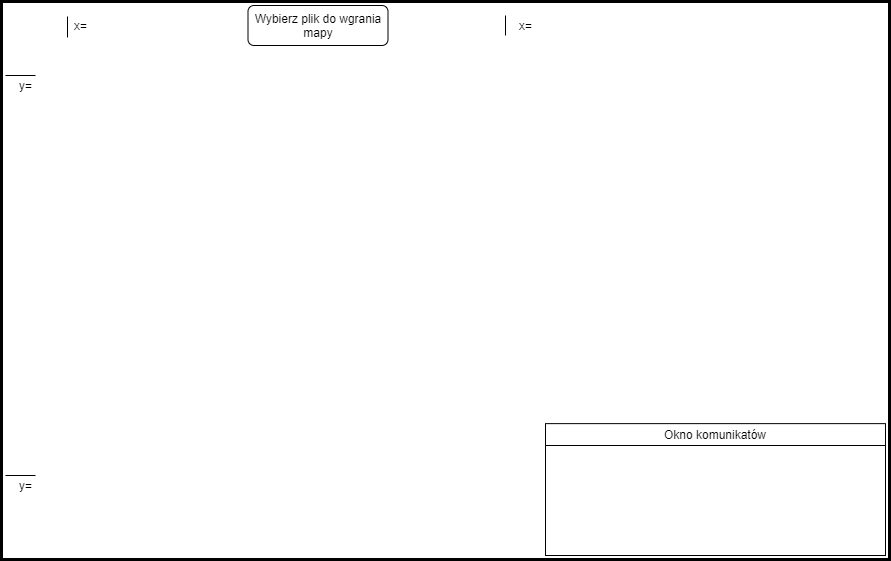
\includegraphics[width=\linewidth]{./images/startowy_widok.png}
  \caption{Widok startowy.}
  \label{fig:GUIstart}
\end{figure}

W prawym dolnym rogu znajduje się okno komunikatów. W górnej części znajduje sie przycisk "wybierz plik do wgrania mapy", kótry należy wciskąć aby wybrać z komputera plik wejściowy z mapą. Dodatkowo widoczne są 4 krótkie odcinki. Dwa pionowe będą oznaczyły skrajne wartości punktów zaznaczonych na mapie w osi x a obok nich pojawią się odpowiadające im wartości. Analogicznie odcinki poziome oznaczają skrajne wartości punktów zaznaczonych na mapie w osi y a obok nich odpowiadające im wartości. Po wgraniu poprawnego pliku pojawia się mapa państwa i dodatkowe przuciski jak na Rysnuku 2.

\begin{figure}[h]
  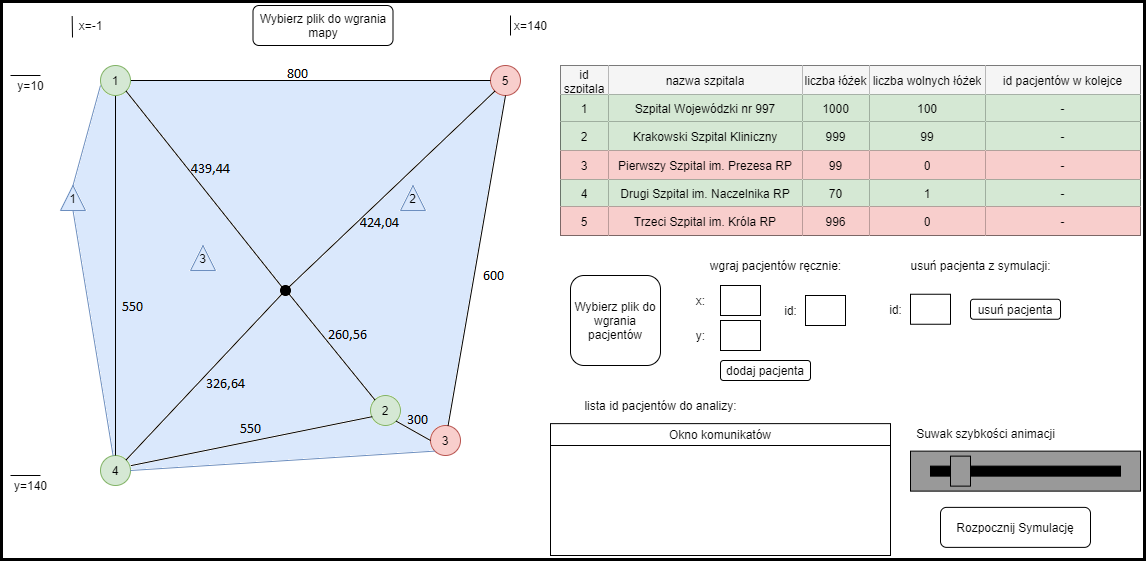
\includegraphics[width=\linewidth]{./images/widok_z_mapa.png}
  \caption{Widok po załadowaniu mapy.}
  \label{fig:GUImap}
\end{figure}

Terytorium państwa ma niebieskie tło. Obikety oznaczono kształtem trójkąta wewnątrz którego znajduje się jego id, które zostało podane w pliku wejściowym. Kołami oznaczono szpitale. Jeśli w danym szpitalu są jeszcze miejsca to jest to koło koloru zielonego w przeciwnym przypadku koło koloru czerwonego. Wewnąrz koła znajduje się numer id zgodny z plikiem wejściowym. Odcinki koloru czarnego na mapie to drogi. Droga na mapie ma początek i koniec w szpitalu lub na skrzyżowaniu. Zatem niektóre drogi z pliku do wgrywania w mapy zostały podzielone na mniejsze z uwagi na skrzyżowania. W okolicy środka każdej drogi została podana wartość jej długości. Czarną kropką zostały oznaczone na mapie skrzyżowania. Po wgraniu mapy pojawiły się skrajne wartości występujące na mapie przy odcinkach które były już widoczne przed załadowaniem mapy.

Po prawej stronie od mapy na samej górze znajduje się tabela, która zawiera rekordy szpitali: ich id, nazwę, liczbę łóżek, liczbę wolnych łóżek i kolejkę pacjentów oczekujących na przyjęcie do danego szpitala. Kolejka składa się z ciągu id pacjentów w kolejce oddzielonych przecinkami. Jeżeli dany szpital nie ma wolnych łóżek wiersz jest w kolorze czerwonym. W przeciwnym przypadku jest koloru zielonego.

Poniżej tabeli z informacjami o szpitalach znajdują się 3 sekcje operacji na pacjentach. Pierwszy z obiekt z lewej to przycisk o nazwie "Wybierz plik do wgrania pacjentów", który służy do wgrywania pliku wejściowego z pacjentami. Druga sekcja składa się z trzech pól do wpisywania liczb oraz przycisku dodaj pacjenta.Aby dodać pacjenta użytkownik musi podać jego współrzędne x, y oraz jego id, a następnie wcisnąć przycisk "dodaj pacjenta". Trzecia sekcja służy do usuwania pacjentów, których jednak nie będziemy chcieli poddawać symulacji. Dla wybranego pacjenta należy wpisać jego id w pole do wpisywania liczb oraz wcisnąć przycisk "usuń pacjenta". Lista id pacjentów, którzy będą podani symulacji po jej uruchomieniu znajduje się nad oknem komunikatów. Kojene id są oddzielane przecinkami a kolejność jest zgodna z kolejnością wprowadzania koljenych pacjentów.

Na prawo od okna kounikatów znajudje się przycisk "Rozpocznij Symylację", który blokuje wprowadznie nowych pacjentów oraz zmianę mapy i dokonuje animacji transportowania pacjentów do szpitala w kolejności jak zostali wprowadzani do programu. Nad przyciskiem "Rozpocznij Symulację" znajduje się suwak regulujący szybkość animacji.

\section{Przebieg animacji}

Po wciśnięciu przycisku "Rozpocznij Symulację" na mapie pokazują wszyscy pacjenci jako pomarańczowe kropki. Następnie każdy kropka oznaczająca pacjenta, według kolejności na liście pacjentów poddawanych symulacji, zaczyna przemieszczać. Dodatkowo zostawia za sobą łamaną w postaci przebytej trasy w kolorze pomarańczowym. Widok takiego przemieszczania się pacjenta oraz pozostałych pacjentów czekających na swoją kolej został pokazany na Rysnuku 3.

\begin{figure}[h]
  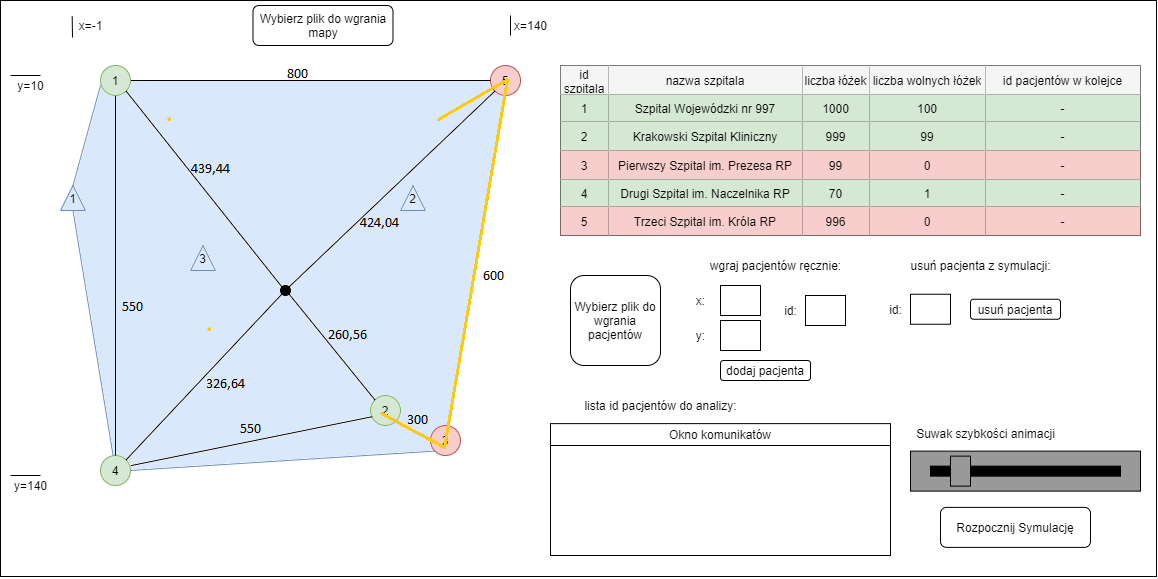
\includegraphics[width=\linewidth]{./images/widok_symulacji.png}
  \caption{Widok symulacji.}
  \label{fig:GUIsym}
\end{figure}

Gdy dany punkt dotrze do szpitala gdzie jest wolne miejsce pojawia się stosowny komunikat informujący o przyjęciu pacjenta o danym id do szpitala o danym id. Następuje aktualizacja liczby wolnych miejsc w danym szpitalu i ewentualnie zmiana jego koloru na mapie i w tabeli na kolor czerwony. Następnie znika punkt symbolizujący dopiero co przyjętego pacjęta z mapy jak róznież znika jego trasa. Dalej jest inicjalizowane rozpoczęcie animacji trasy kolejnych pajentów. Jeżeli dla danego pacjenta nie starczy miejscaa w żadnym szpitalu to pojawia się o tym komunikat w oknie komunikatów. Napstępnie id tego pacjenta jest dodawane w tabeli szpiatali do listy id pacjentów w kolejce. Następnie znika punkt i jego trasa i rozpoczyna sie symulacja kolejnego pacjenta. Jeżeli jakiś pacjent jest poza granicami państwa to pojawia się o tym komunikat. Następnie znika on z mapy i następuje animacja kolejnego pacjenta. Gdy już wszysycy pacjenci dostali poddani symulacji w oknie komunikatów pojawia sie komunikat o zakończeniu symulacji. Dalej program ma zapisane w pamięci mapę i pacjetnów i można dowolnie wiele razy wykonywać symulację. Aby zakończyć działanie programu należy wycisnąć przycisk ESC.

\section{Możliwe komunikaty w oknie komunikatów}
Gdy plik wejściowy jest niezgodny z opisem z rozdziału 2. lub zostanie podana błędna ścieżka do tego pliku lub on nie istnieje, to program nie wykona swojego zadania a w terminalu pojawi się błąd. Rodzaj komunikatu będzie zależał od tego co zostało źle zrobione. Poniżej wypunktowano możliwe błędy i ich komunikaty:
\begin{itemize}
\item brak parametru w komendzie uruchamiającej program w postaci ścieżki do pliku wejściowego:\\ \textbf{Error: not given input file name}
\item brak pilku wejściowego lub niepoprawna ścieżka dostępu do niego:\\ 			\textbf{Error: input file not found}
\item błędny znak w pliku tekstowym: \\ \textbf{Error in line \textless numer linii\textgreater: incorrect char in input file}
\item brak nagłówka rozpoczynającego się znakiem \# :\\ \textbf{Error in line \textless numer linii\textgreater: no section header}
\item brak danych (jakiejkolwiek linii) w którejś sekcji: \\ \textbf{Error in line \textless numer linii\textgreater: no data in this section}
\item brak jednej z pozycji w danych: \\ \textbf{Error in line \textless numer linii\textgreater: missing data}
\item znak "$\mid$" po ostatniej spodziewanej pozycji danych: \\ \textbf{Error in line \textless numer linii\textgreater: to many $\mid$ chars}
\item niezgodny typ danych: \\ \textbf{Error in line \textless numer linii\textgreater: unexpected type of data}
\item liczba jest ujemna gdy wymagana jest nieujemna: \\ \textbf{Error in line \textless numer linii\textgreater: the given value should not be negative}
\item liczba jest niedodatnia, gdy wymagana jest dodatnia: \\ \textbf{Error in line \textless numer linii\textgreater: the given value should be positive}
\item id nie jest unikalne: \\ \textbf{Error in line \textless numer linii\textgreater : the id is not unique }
\item w połączeniach jest użyte id, które nie istnieje: \\ \textbf{Error in line \textless numer linii\textgreater: the id does not fit any object}
\item w połączeniach użyto dwukrotnie (lub więcej) tej samej kombinacji id apteki i producenta: \\ \textbf{Error in line \textless numer linii\textgreater : connection between this pharmacy and manufacturer has been already set}
\item koszt jednej szczepionki jest podany z trzema lub więcej cyframi po przecinku: \\ \textbf{Error in line \textless numer linii\textgreater: the cost of one vaccine is incorrect}
\item liczba połączeń nie równa się iloczynowi liczby aptek i producentów: \\ \textbf{Error: missing connections between pharmacy and manufacturer}
\end{itemize}

\section{Źródła}
Wykorzystane przykłady pliku wejściowego z mapą i pliku wejścowego z pacjentami są stworzone przez Pawła Zawadzkiego z Wydziału Elektrycznego Politechniki Warszawskiej w 2020 roku.

\end{document}{article}


